\paragraph{QuizziPedia::Front-End::Views::CreateWithWizardView}
\begin{figure} [ht]
	\centering
	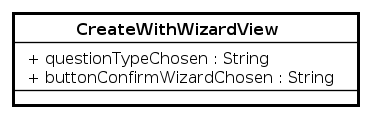
\includegraphics[scale=0.80]{UML/Classi/Front-End/QuizziPedia_Front-end_Views_CreateWithWizardView.png}
	\caption{QuizziPedia::Front-End::Views:CreateWithWizardView}
\end{figure} \FloatBarrier
\begin{itemize}
	\item \textbf{Descrizione}: \textit{view\ped{G}} per la creazione di una domanda tramite wizard;
	\item \textbf{Utilizzo}: permette all'utente di creare una domanda attraverso l'utilizzo di un wizard;
	\item \textbf{Relazioni con altre classi}:
	\begin{itemize}
		\item \textbf{IN \texttt{CreateWithWizardModelView}}: classe di tipo modelview la cui istanziazione è contenuta all'interno della variabile di ambiente \texttt{\$scope} di \textit{Angular\ped{G}}. All'interno di essa sono presenti le variabili e i metodi necessari per il \textit{Two-Way Data-Binding\ped{G}} tra la \textit{view\ped{G}} \texttt{CreateWithWizardView} e il \textit{controller\ped{G}} \texttt{CreateWithWizardController};
		\item \textbf{IN \texttt{LangModel}}: rappresenta il modello delle informazioni per la giusta traduzione dell'applicazione.
	\end{itemize}
		\item \textbf{Attributi}:
		\begin{itemize}
			\item \texttt{+ questionTypeChosen: String} \\ Attributo che specifica la tipologia di wizard da mostrare all'utente a seconda della tipologia di domanda da creare da lui scelta;
			\item \texttt{+ buttonConfirmWizardChosen: String} \\ Attributo che viene utilizzato per visualizzare la giusta traduzione della \textit{label\ped{G}} per il bottone di conferma, in italiano o in inglese; 
		\end{itemize}
\end{itemize}